% Beamer template
% Author: Ozgur Taylan TURAN
% Delft University of Technology

\documentclass[aspectratio=169]{beamer}
% PACKAGES
\usepackage[english]{babel}
\usepackage{graphicx}
\usepackage{animate}
%\usepackage{calc}
\usepackage{calligra}
\usepackage[absolute,overlay]{textpos}
\usepackage[T1]{fontenc}
%\usefonttheme{serif}
\usefonttheme{professionalfonts}
\usepackage{amsmath}
\usepackage{palatino}
\usepackage{mathpazo}
\usepackage{graphicx}
%\usepackage{subfig}
\usepackage{tikz}
\usepackage{ctable}
\usetikzlibrary{shapes,arrows}
\usepackage{xcolor}
\usepackage[T1]{fontenc}
%\usefonttheme{serif}
%\usepackage{titling}
\usepackage{graphicx}
%\usepackage{subfig}
%\usepackage{tikz}
%\usetikzlibrary{shapes,arrows}
\usepackage{mathtools}
\usepackage{cancel}
\graphicspath{D:/LATEX/Reports@IIT/figures}
% CUSTOM PACKAGES
\usepackage{/home/taylanot/texmf/tex/beamerthemetot}
\input{/home/taylanot/texmf/presentation/tune.tex}
% COVER PAGE INFO   
\newcommand{\mytitle}{\color{White}\huge{\textbf{Coffee Talk \#9}}}
\newcommand{\mysubtitle}{\color{Pink}\Large{\textbf{Modeling Machine Learning Multiverse}}}
\newcommand{\myauthor}{\color{White}\textcalligra{\LARGE Ozgur Taylan Turan}}
\newcommand{\authorlabel}{\small O.T. Turan}
\author{\authorlabel}

\newcommand{\R}{\mathbb{R}}
\newcommand{\E}{\mathbb{E}}
\newcommand{\D}{\mathcal{D}}
\newcommand{\A}{\mathcal{A}}
\DeclareMathOperator*{\argmin}{arg\,min}
\begin{document}
% COVER PAGE

{
\def\beamer@entrycode{\vspace*{-\headheight}}
\setbeamertemplate{frametitle}[default][center]
\setbeamertemplate{navigation symbols}{}
\usebackgroundtemplate{
\includegraphics[width=\paperwidth,height=\paperheight]{cover/coverart.pdf}}

\begin{frame}[plain] 

\begin{minipage}{\textwidth}
	\centering{\mytitle} \\
	%\vspace{1cm}
	%\centering{\mysubtitle} \\
	\vspace{1cm}
	\centering{\color{White}November 15, 2021} \\
	\vspace{1cm}
	\centering{\myauthor}\\
\end{minipage}
\end{frame}
}


\begin{frame}
  \begin{minipage}{0.3\textwidth}
    \centering
    
\includegraphics[width=\textwidth]{figures/movie.jpeg}
  \end{minipage}%
  \begin{minipage}{0.7\textwidth}
  \centering
  \mysubtitle\cite{bell2022}
  \end{minipage}

\end{frame}

\begin{frame}{Why this paper?}
  \centering
  \begin{itemize}
    \item Interesting effort...
  \end{itemize}
\end{frame}

\begin{frame}{Aim}
  \centering
  \begin{itemize}
    \item Present a principled framework for backed up claims...
    \item A step closer to reproducibility...
  \end{itemize}
\end{frame}

\begin{frame}{Introduction}
  \begin{minipage}{0.5\textwidth}
    \only<1> 
    {
      \color{Pink} Multiverse Analysis \cite{steegen2016}
      \begin{itemize}
        \item Psychology background...
        \item Make all the possible choices at the same time!
        \item Mostly related to dataset construction.
        \item Different choices affect the outcome/conclusion!
      \end{itemize}
    }
  \end{minipage}%
  \begin{minipage}{0.5\textwidth}
    \only<2> 
    {
      \color{Pink} Machine Learning
      \begin{itemize}
        \item Again possible choices (batch size, learning rate architecture etc.) 
        \item CLAIM: With this method we can investigate the effect of each choice...
      \end{itemize}
    }
  \end{minipage}
\end{frame}

\begin{frame}{Multiverse Exploration}
  \only<1>
  {
  \color{Pink} \textbf{search space} $\mathcal{X}$ (claim: often continuous) and \textbf{evaluation function} $l$ $\to$ multiverse 
  \color{Black} Due to search space being too large $\to$ GP surrogate and explore the space using Bayesian experimental design!
  }
  \only<2>
  {
  \begin{itemize}
    \item Sample initial design $X_0\sim\mathcal{X}$ and evaluate $Y_0=l(X0)$ [They select Sobol sequence as initial design]
    \item Fit a GP model to $X_0$ and $Y_0$
    \item Use acquisition function $a$ on $f$ to sample and evaluate a new batch $(X_i,Y_i)$
    \item Repeat until a stopping criterion... [Bayes factor:=$\frac{P(X,Y|K_shared)}{P(X,Y|K_additive)}$]
    \item Sensitivity analysis
  \end{itemize}
  }
  \only<3>
  {
  Caveat:
  \begin{itemize}
    \item $a$ Integrated Variance Reduction $\to$ nasty integral $\to$ Monte-Carlo approx.
    \item Difference with standard optimization!
  \end{itemize}
  }
\end{frame}

\begin{frame}{Optimization vs Exploration}
  \centering
  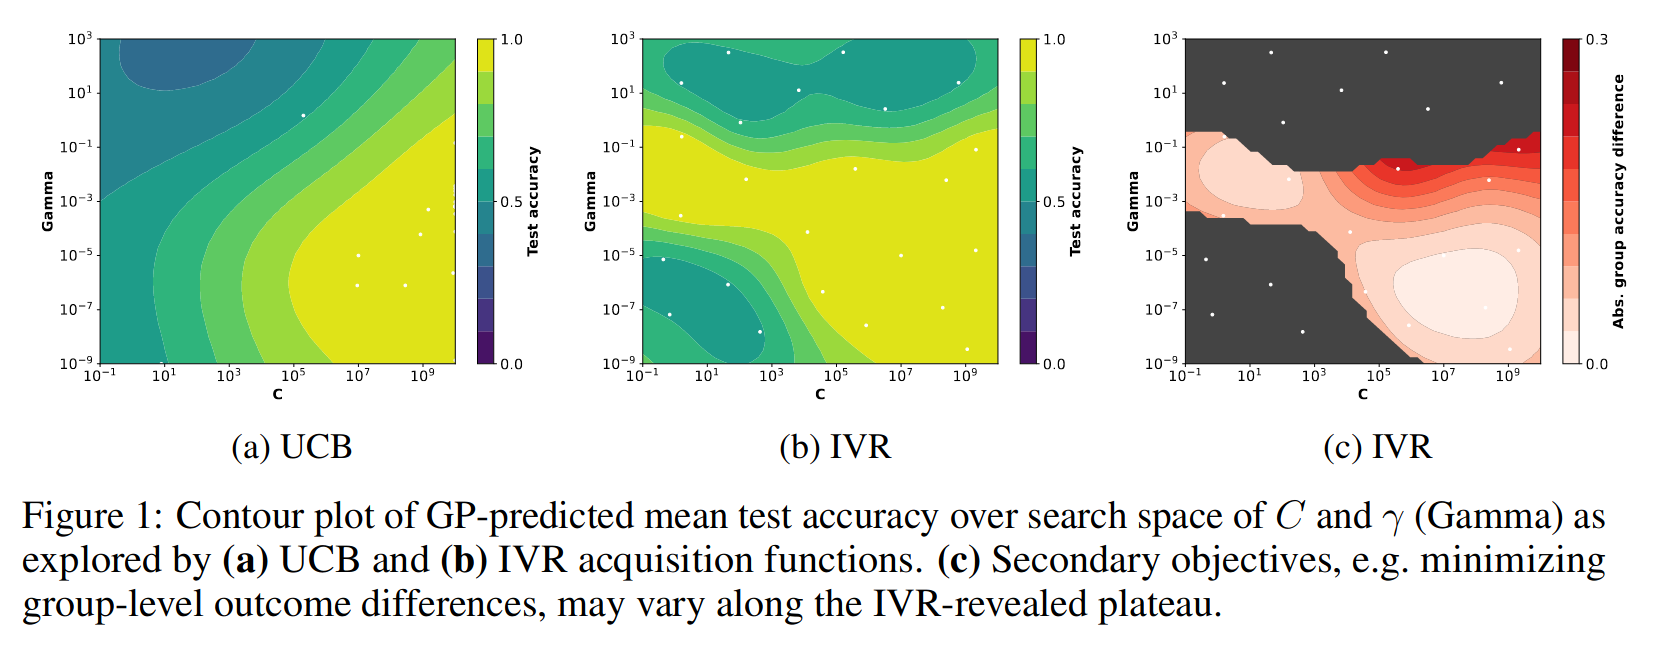
\includegraphics[width=0.8\textwidth]{figures/svm.png}
  \begin{itemize}
    \item Premature optimization hinders our understanding...
    \item Not to throw shade at optimization!
  \end{itemize}
\end{frame}

\begin{frame}{When is Adaptive optimization helpful?}
  \centering
  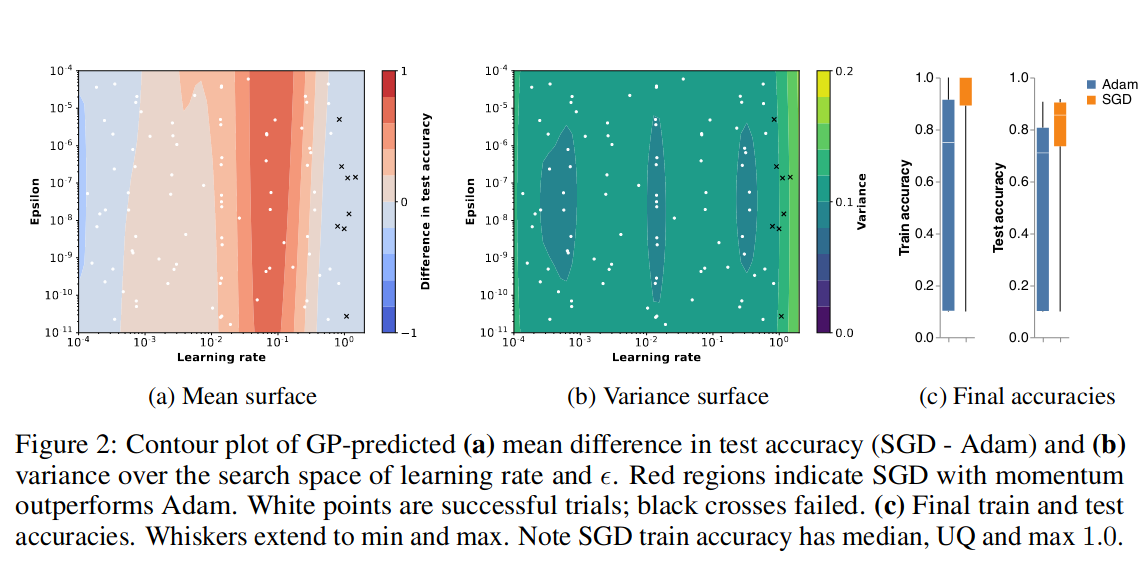
\includegraphics[width=0.65\textwidth]{figures/optim.png}
  \begin{itemize}
    \item SGD with momentum vs Adam
    \item Opposing the claims of \cite{wilson2018} SGD>Adam
  \end{itemize}
\end{frame}

\begin{frame}{Is there a large-batch generalization gap?}
  \begin{minipage}{0.55\textwidth}
    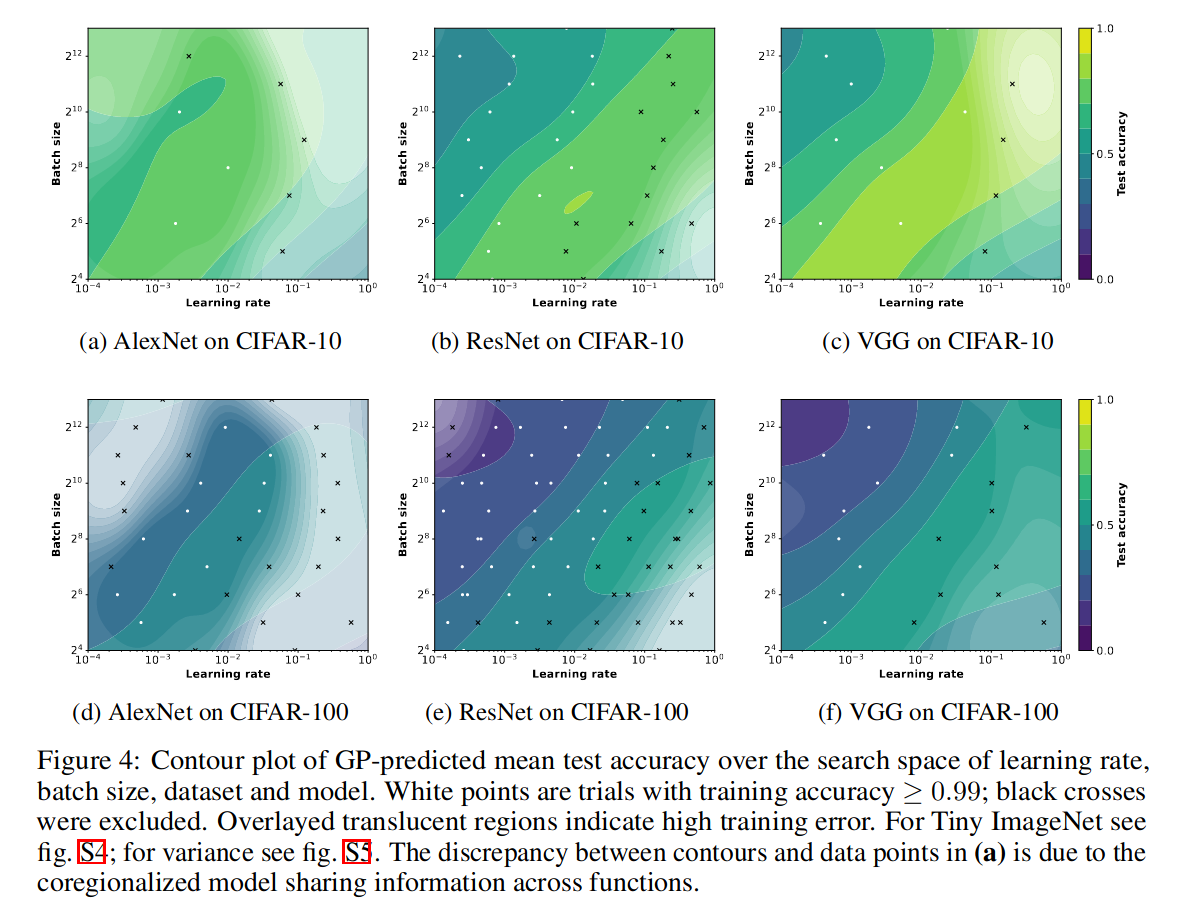
\includegraphics[width=\textwidth]{figures/batch.png}
  \end{minipage}%
  \begin{minipage}{0.45\textwidth}
  \begin{itemize}
    \item Many Researchers: batch size $\uparrow$ $\to$ generalization $\downarrow$
    \item Batch-size by itself does not explain the generalization performance! 
  \end{itemize}
  \end{minipage}
\end{frame}

\begin{frame}{Conclusions}
  \centering
  \begin{itemize}
    \item By using a multiverse analysis, researchers and practitioners gain more robust claims and better understanding of the consequences of their decisions.
  \end{itemize}
\end{frame}

\begin{frame}
    \color{Pink} 
    \centering
     THANKS!
\end{frame}


\end{document}

